%% $RCSfile: proj_report_outline.tex,v $
%% $Revision: 1.3 $
%% $Date: 2016/06/10 03:41:54 $
%% $Author: kevin $

\documentclass[11pt
              , a4paper
              , oneside
              ]{report}


\usepackage{float} % lets you have non-floating floats
\usepackage{url} % for typesetting urls
\usepackage{graphicx}
\usepackage{subcaption}
\usepackage[table,xcdraw]{xcolor}
\usepackage{hyperref}
\usepackage{titlesec}

\setlength{\parindent}{0pt}

\usepackage{titlesec}
\titleformat{\chapter}[hang] 
{\normalfont\huge\bfseries}{\chaptertitlename\ \thechapter:}{1em}{} 

%
%  We don't want figures to float so we define
%
\newfloat{fig}{thp}{lof}[chapter]
\floatname{fig}{Figure}

%% These are standard LaTeX definitions for the document
%%                            
\title{Instrumentation System for Liquid Drop Impact and Evaporation}
\author{Daniel Eisen}

%% This file can be used for creating a wide range of reports
%%  across various Schools
%%
%% Set up some things, mostly for the front page, for your specific document
%
% Current options are:
% [ecs|msor|sms]          Which school you are in.
%                         (msor option retained for reproducing old data)
% [bschonscomp|mcompsci]  Which degree you are doing
%                          You can also specify any other degree by name
%                          (see below)
% [font|image]            Use a font or an image for the VUW logo
%                          The font option will only work on ECS systems
%
\usepackage[image,ecs]{vuwproject}

% You should specifiy your supervisor here with
\supervisor{Dr. Gideon Gouws}
% use \supervisors if there is more than one supervisor

\otherdegree{Bachelor of Engineering with Honours}

% Unless you've used the bschonscomp or mcompsci
%  options above use
%   \otherdegree{OTHER DEGREE OR DIPLOMA NAME}
% here to specify degree

% Comment this out if you want the date printed.
\date{}


\begin{document}

% Make the page numbering roman, until after the contents, etc.
%\frontmatter

%%%%%%%%%%%%%%%%%%%%%%%%%%%%%%%%%%%%%%%%%%%%%%%%%%%%%%%

%%%%%%%%%%%%%%%%%%%%%%%%%%%%%%%%%%%%%%%%%%%%%%%%%%%%%%%

\begin{abstract}
    //TODO rewriting
    
    \textit{Droplet impact and evaporation presents a complex physical process worth investigating not only from a fundamental research perspective but also in its potential for industrial application. However, in order to extract usable data from this small scale, fast phenomenon in the lab producing a droplet of repeatable volume and position as well as accucartly track and collect the data (temperature, impact, evaporation) is essential in order to extract reliable and study worthy results. This procedure form the basis of this project.
    This projects approach is to add motorised automation to droplet dispensing with aims to control for droplet volume, positional variation, contact angle and speed up the procedure and allow for greater flexibility in the experimental process.}


\end{abstract}

%%%%%%%%%%%%%%%%%%%%%%%%%%%%%%%%%%%%%%%%%%%%%%%%%%%%%%%

\maketitle

\tableofcontents

%%%%%%%%%%%%%%%%%%%%%%%%%%%%%%%%%%%%%%%%%%%%%%%%%%%%%%%

\mainmatter

%%%%%%%%%%%%%%%%%%%%%%%%%%%%%%%%%%%%%%%%%%%%%%%%%%%%%%%

% individual chapters included here
\chapter{Introduction}\label{C:intro}
The investigation of droplet impact and evaporation is an area of interest and application to various industries. Examples of these include milk powder spray drying, ink jet printing, and applications of evaporative cooling. This project will continue on from a previous instrumentation setup, evaluating its shortcomings, and designing the next generation. This will improve the reliability and usability of the collected data from the previous setup, and introduce methods of automating the process. 

This preliminary report covers the key problem of the experimental setup that the project aims to improve, and identifying the main factors that can introduce variation into the results. It will also provide an overview and evaluation of the current and previous systems, and the variability of their results, including possible sources of these inconsistencies. It will briefly cover other similar systems in literature, and what they control and how. Then the report will redefine the project scope, its objectives, and what variables it aims to control and how. Finally, it will cover what work has been done and where the current progress and results stand, as well as detailing difficulties and decisions made along the way.  

\section*{The Experiment}

A droplet of liquid (concentrated milk, water, or similar) is deposited on a heated substrate (stainless steel, copper, or glass). The temperature of the substrate is monitored. The progression of the droplet's impact and evaporation is captured by two cameras; above and profile view. This produces a multidimensional perception of the developing behaviour and characteristics of the droplet over time. This usually takes between 1 and 2 minutes per droplet.

\subsection*{Problems}

This experiment relies on the precise placement of a droplet above a temperature sensor, in a set focal plane, to measure the droplet as it progresses through it's evaporation.
Therefore, it can be said there exists uncontrolled factors that can alter the results, affecting the final values and the repeatability of the experiment.
These factors can be separated into environmental and procedural sources.

\begin{table}[h]
    \centering
    \begin{tabular}{|l|l|}
    \hline
    \multicolumn{1}{|c|}{\textbf{Environmental}} & \multicolumn{1}{c|}{\textbf{Procedural}} \\ \hline
    Humidity                                     & Droplet Volume                          \\ \hline
    Atmospheric Pressure                        & Droplet Position (Rel. to thermocouple) \\ \hline
    Temperature                                  & Contact Angle (contact surface area)    \\ \hline
    \end{tabular}
    \end{table}
\chapter{Background}\label{C:back}
\begin{itemize}
    \item Outline the main topic and problem of droplet experiment
\end{itemize}
\section{Evaluation of Previous System}

\section{Other Solution in Literature}

\section{Background on Stepper motor control}
\begin{itemize}
    \item This will be relevant when discussing design decisions made in work chapter
\end{itemize}

\section{Summary}
\chapter{Initial Evaluation}\label{C:init_eval}

\section{Initial Experimental Setup at Project Start}
Given that the express purpose of the project is the development of a new version of instrumentation, the first step is an examination of the prior system. This is to identify how it falls short and to determine the areas that the project will focus on.

The experimental method concerns depositing a liquid droplet upon a heated substrate. The data of note is the temperature evolution of the substrate directly under the drop, as well as image data capturing the point of impact and how the droplet changes over the course of the evaporation.

\vspace*{-16pt}
\begin{figure}[h]
    \begin{center}
        \includegraphics[width=.6\textwidth]{img/init_syr.png}
        \caption{Initial Experimental Setup}
        \label{fig:prior_exp}
    \end{center}
\end{figure}
\vspace*{-16pt}

The prior system uses an optical breadboard and micrometer adjustable stages as mounting platforms and positional control.
A central stage holds the substrate stack, consisting of an aluminium heat-spreader, Peltier heater, and metallic substrate (copper, stainless steel, etc) with an internally mounted thermocouple.
To capture the image data, a pair of manual focus cameras are positioned/suspended in profile and top-down view and are controlled via a USB connection. The thermocouple is sampled with LabVIEW via a USB DaQ.
Dispensing the droplet itself is done by hand using a syringe mounted to another optical stage [\ref{fig:prior_exp}] with XYZ+R controls. It is rotated above the substrate and pressed to dispense a drop.

This would be perfectly fine, however, the results this manual process yields had a level of inconsistency. Thus motivating the design of a new system to control for the experiments variation.

\section{Repeatability and Reliability}
To identify more precisely the drawbacks in the performance of the prior setup and inform the requirements of the project, previously collected data was first analysed.

The data was taken from a series of five droplet runs, and was analysed to quantify the repeatability and reliability of the system and to compare the effect of the drop morphology and position with the resulting temperature evolution.

\begin{figure}[h]
    \centering
    \includegraphics[width=.4\textwidth]{img/droplets_2018.png}
    \includegraphics[width=.4\textwidth]{img/drop_pos_2018.png}
    \caption{Droplet positional and shape variation; Left: Camera overlay, Right: Quantified Offsets [mm $\angle$ degrees]}
    \label{fig:init_pos}
\end{figure}

The first analysis is the image data. The substrate itself has a mark to represent the position of the thermocouple, this is used as the main reference to quantify the droplet position. Reference images set calibration at 120.14 pixels/mm and 109.2 pixels/mm for the top down and profile cameras respectively, and was used to measure the droplet centre offset and angle (from the reference point) as well as the height, width and contact angles of the droplet on the substrate.

As seen above, the quite substantial positional variation between the runs. Ranging [0.71:2.01]mm offset and [-16:-123]$^\circ$ angle.


\begin{equation}
    \frac{1}{6}\pi h(3a^2 + h^2)
    : a \equiv \mathrm{half \; width}, \; h \equiv \mathrm{height}
    \label{equ:vol}
\end{equation}
From the data extracted from the profile camera (height, width, contact angle) the volume of the droplets could be estimated. The method chosen was of the represent the droplet as a spherical cap and use the above equation \ref{equ:vol}to compute it.

\begin{figure}[h]
    \centering
    \includegraphics[width=.4\textwidth]{img/drop_temps_2018.png}
    \includegraphics[width=.4\textwidth]{img/2018_pos_temp_trend.png}
    \caption{Left: Initial Systems temperature data showing large relative variation, Right: Drop offset magnitude (mm) against resulting measured temperature drop}
\end{figure}

By taking a series of consecutively collected temperature data using the initial system the observed variation can be quantified. As a pre-processing step a 1sec rolling average is applied to the collected vectors. They are then time aligned to zero at the point of droplet contact, indicated by a sudden temperature drop. This data is then transformed into a temperature delta relative to the temperature just before contact. 

Observed is $0.112^\circ C$ variance between the initial temperature drops between all runs and all runs are observed to evolve at differing rates, rebounding to drifting temperatures etc. This is the main justifying factor in perusing an improved instrumentation system.   

\newpage
\section{Summary}

\begin{table}[h]
    \centering
    \begin{tabular}{|l|l|l|l|}
        \hline
        \textit{\textbf{Droplet}}                          & \textit{Offset(mm)} & \textit{Volume(uL)} & \textit{delta T (c)}\\ \hline
        \cellcolor[HTML]{9698ED}1                          & 0.7506              & 16.55               &  -1.649861        \\ \hline
        \cellcolor[HTML]{E9AD3F}2                          & 0.7164              & 17.91               &  -1.790142        \\ \hline
        \cellcolor[HTML]{C0C0C0}3                          & 0.9402              & 17.89               &  -1.294989        \\ \hline
        \cellcolor[HTML]{FFFC9E}4                          & 2.0104              & 17.57               &  -0.994441        \\ \hline
        \cellcolor[HTML]{79CD5D}5                          & 0.8258              & 16.21               &  -1.712207        \\ \hline
        \cellcolor[HTML]{FFFFFF}\textbf{\textit{Variance}} & \textit{0.2964}     & \textit{0.6288}     &  \textit{0.1121527 }       \\ \hline
    \end{tabular}
\end{table}

To summarise the results of this initial evaluation, a variance of the droplets morphology and resulting temperature measurement are taken and used as a guide for the projects specification and comparative evaluation.    

To fully guide and justify the direction this project will take in attempting to improve this experiment it will consider and address a list of possible affecters on the experiment results.

\begin{table}[h]
    \centering
    \begin{tabular}{|l|l|l|}
        \hline
        \textbf{Effector} & \textbf{Likelihood} & \textbf{Effect Strength} \\ \hline
        Position          & HIGH                & HIGH                     \\ \hline
        Volume            & MODERATE            & HIGH                     \\ \hline
        Contact angle*    & MODERATE            & MODERATE                     \\ \hline
        Humidity          & LOW                 & HIGH                     \\ \hline
        Temperature       & LOW                 & HIGH                     \\ \hline
        Pressure          & MODERATE            & MODERATE                 \\ \hline
    \end{tabular}
\end{table}
\textit{\small{*Contact angle is more a function of the surface cleaning of the substrate, and is only representative of the surface area of contact with the substrate}} \\

Droplet position is a result of the method of dispensing and as seen in figure 3.3 correlates to variation in the observed temperature data collected via the substrates embedded thermocouple. Due to the manual method of dispensing, this variation is very likely to occur and is essentially uncontrolled in the initial experiment other than a reference point as a target. 
The volume and Contact angle of the droplet is more a result of procedural inconsistencies. The volume being a factor of the syringe and contact angle being very dependant of the surface finish/quality/cleaning of the substrate.

The environmental factors differ from these, as the experiment is carried out in a climate-controlled lab there are very few high-frequency changes but these factors can greatly affect the rate of evaporation of the droplet.

Given the above, this project will focus on the controlling the procedural affecters but will supply a method for collecting data on the environmental affecters for analysis.
\chapter{Design}\label{C:design}

The design process uses the goals of the experiment and the results of the initial evaluation to inform what and how various subsystems are designed.

From this there is a number of requirements to consider:

\begin{itemize}
    \item \textbf{Mechanical Stability}:
    \item \textbf{System Expandability}:
    \item \textbf{text}
\end{itemize}

\section{System Overview}

\begin{figure}[h]
    \begin{center}
        \includegraphics[width=0.5\textwidth]{img/ED_block_diag.png}
    \end{center}
\end{figure}

\section{Mechanical Design}

\subsection{Rotating Pipette Mount}

\subsection{Z micrometer Control}

\section{Electronic Design}

\subsection{Motor Driving}

\subsubsection*{The Requirements}
To drive the selected stepper motors, discrete step/direction style micro stepping drivers were chosen. This allows for the design to be flexible with its electronics placed to accommodate the experimental needs. Allows for a fairly agnostic choice for controller to supply the control signals, and standardised pinouts allow for requirement flexibility and replacements.

\begin{table}[h]
    \centering
    \begin{tabular}{|l|l|l|l|l|}
        \hline
        \textbf{}     & \textbf{A4988} & \textbf{DRV8825} & \textbf{STPIN820} & \textbf{DRV8834} \\ \hline
        Step Res      & 1/16           & 1/32             & 1/256             & 1/32             \\ \hline
        Logic Level   & 3V3/5V         & 3V3/5V           & 3V3/5V            & 3V3/5V           \\ \hline
        Current Limit & 1A             & 1.5A             & 0.9A              & 1.5A             \\ \hline
        Drive Voltage & 8-35V          & 8.2-45V          & 7-48V             & 2.5-10.8         \\ \hline
    \end{tabular}
    \caption{Comparison of considered drivers}
\end{table}

Main consideration for device choice are: micro step resolution, driving current limit (passively cooled), and configuration pinout.

\subsubsection*{The Choice}
The DRV8825 was ultimately chosen.
\begin{itemize}
    \item High microstepping resolution, lower than the STPIN820 but cheap high resolution driver are prone to step skipping \cite{step_book}
    \item Highest driving current as torque requirements are unknown for this design the headroom is nice even if it isn't use, especially as it will run cooler at lower power draw.
    \item It ranked above the DRV8834 due to it configuration pins (to set microstepping mode) as it provide all 3 pins without the requirement to leave pins floating as a setting thus allowing for full software control.
\end{itemize}

\subsection{Pipette Triggering}

\subsection{Environmental Monitoring}

\chapter{Implementation}\label{C:imp} 


//TODO rename sections to reflect work done
\section{Mechanical Design}

\begin{itemize}
    \item Go into 3d printing/laser cutting refinement, testing and adjustment
    \item Tolerance and dimension adjustment
    \item Noted changed and drawback from design  
\end{itemize}

\subsection{Rotating Pipette Mount}

\subsection{Z micrometer Control}
\begin{itemize}
    \item Note initially large vibrations as z decreases, caused be loose tolerance, too small coupler. Caused droplet to prematurely detach at larger values.  
\end{itemize}


\begin{figure}[h]
    \centering
    \includegraphics[width=0.4\textwidth]{img/full_sys.jpg}
    \includegraphics[width=0.4\textwidth]{img/impl_sys_top.jpg}
    \includegraphics[width=0.4\textwidth]{img/impl_coup.jpg}
    \includegraphics[width=0.4\textwidth]{img/new_stack.jpg}
\end{figure}

\section{Software}

//Insert Serial Command Table (maybe only appendix)

\subsection{Motorised Dispensing Controller}
ESP32 based system controller with serial interface for issuing commands. Provides functionality to:
\begin{itemize}
    \item Motorised stages, height and angular position
    \item e-Pipette droplet dispensing 
\end{itemize}

\subsection{Environmental Monitor}

\begin{itemize}
    \item Auto sleeping, button wake upon
    \item Circuit-Python implementation
\end{itemize}

\subsection{LabView Temperature Logger}

\section{Electronic Design}

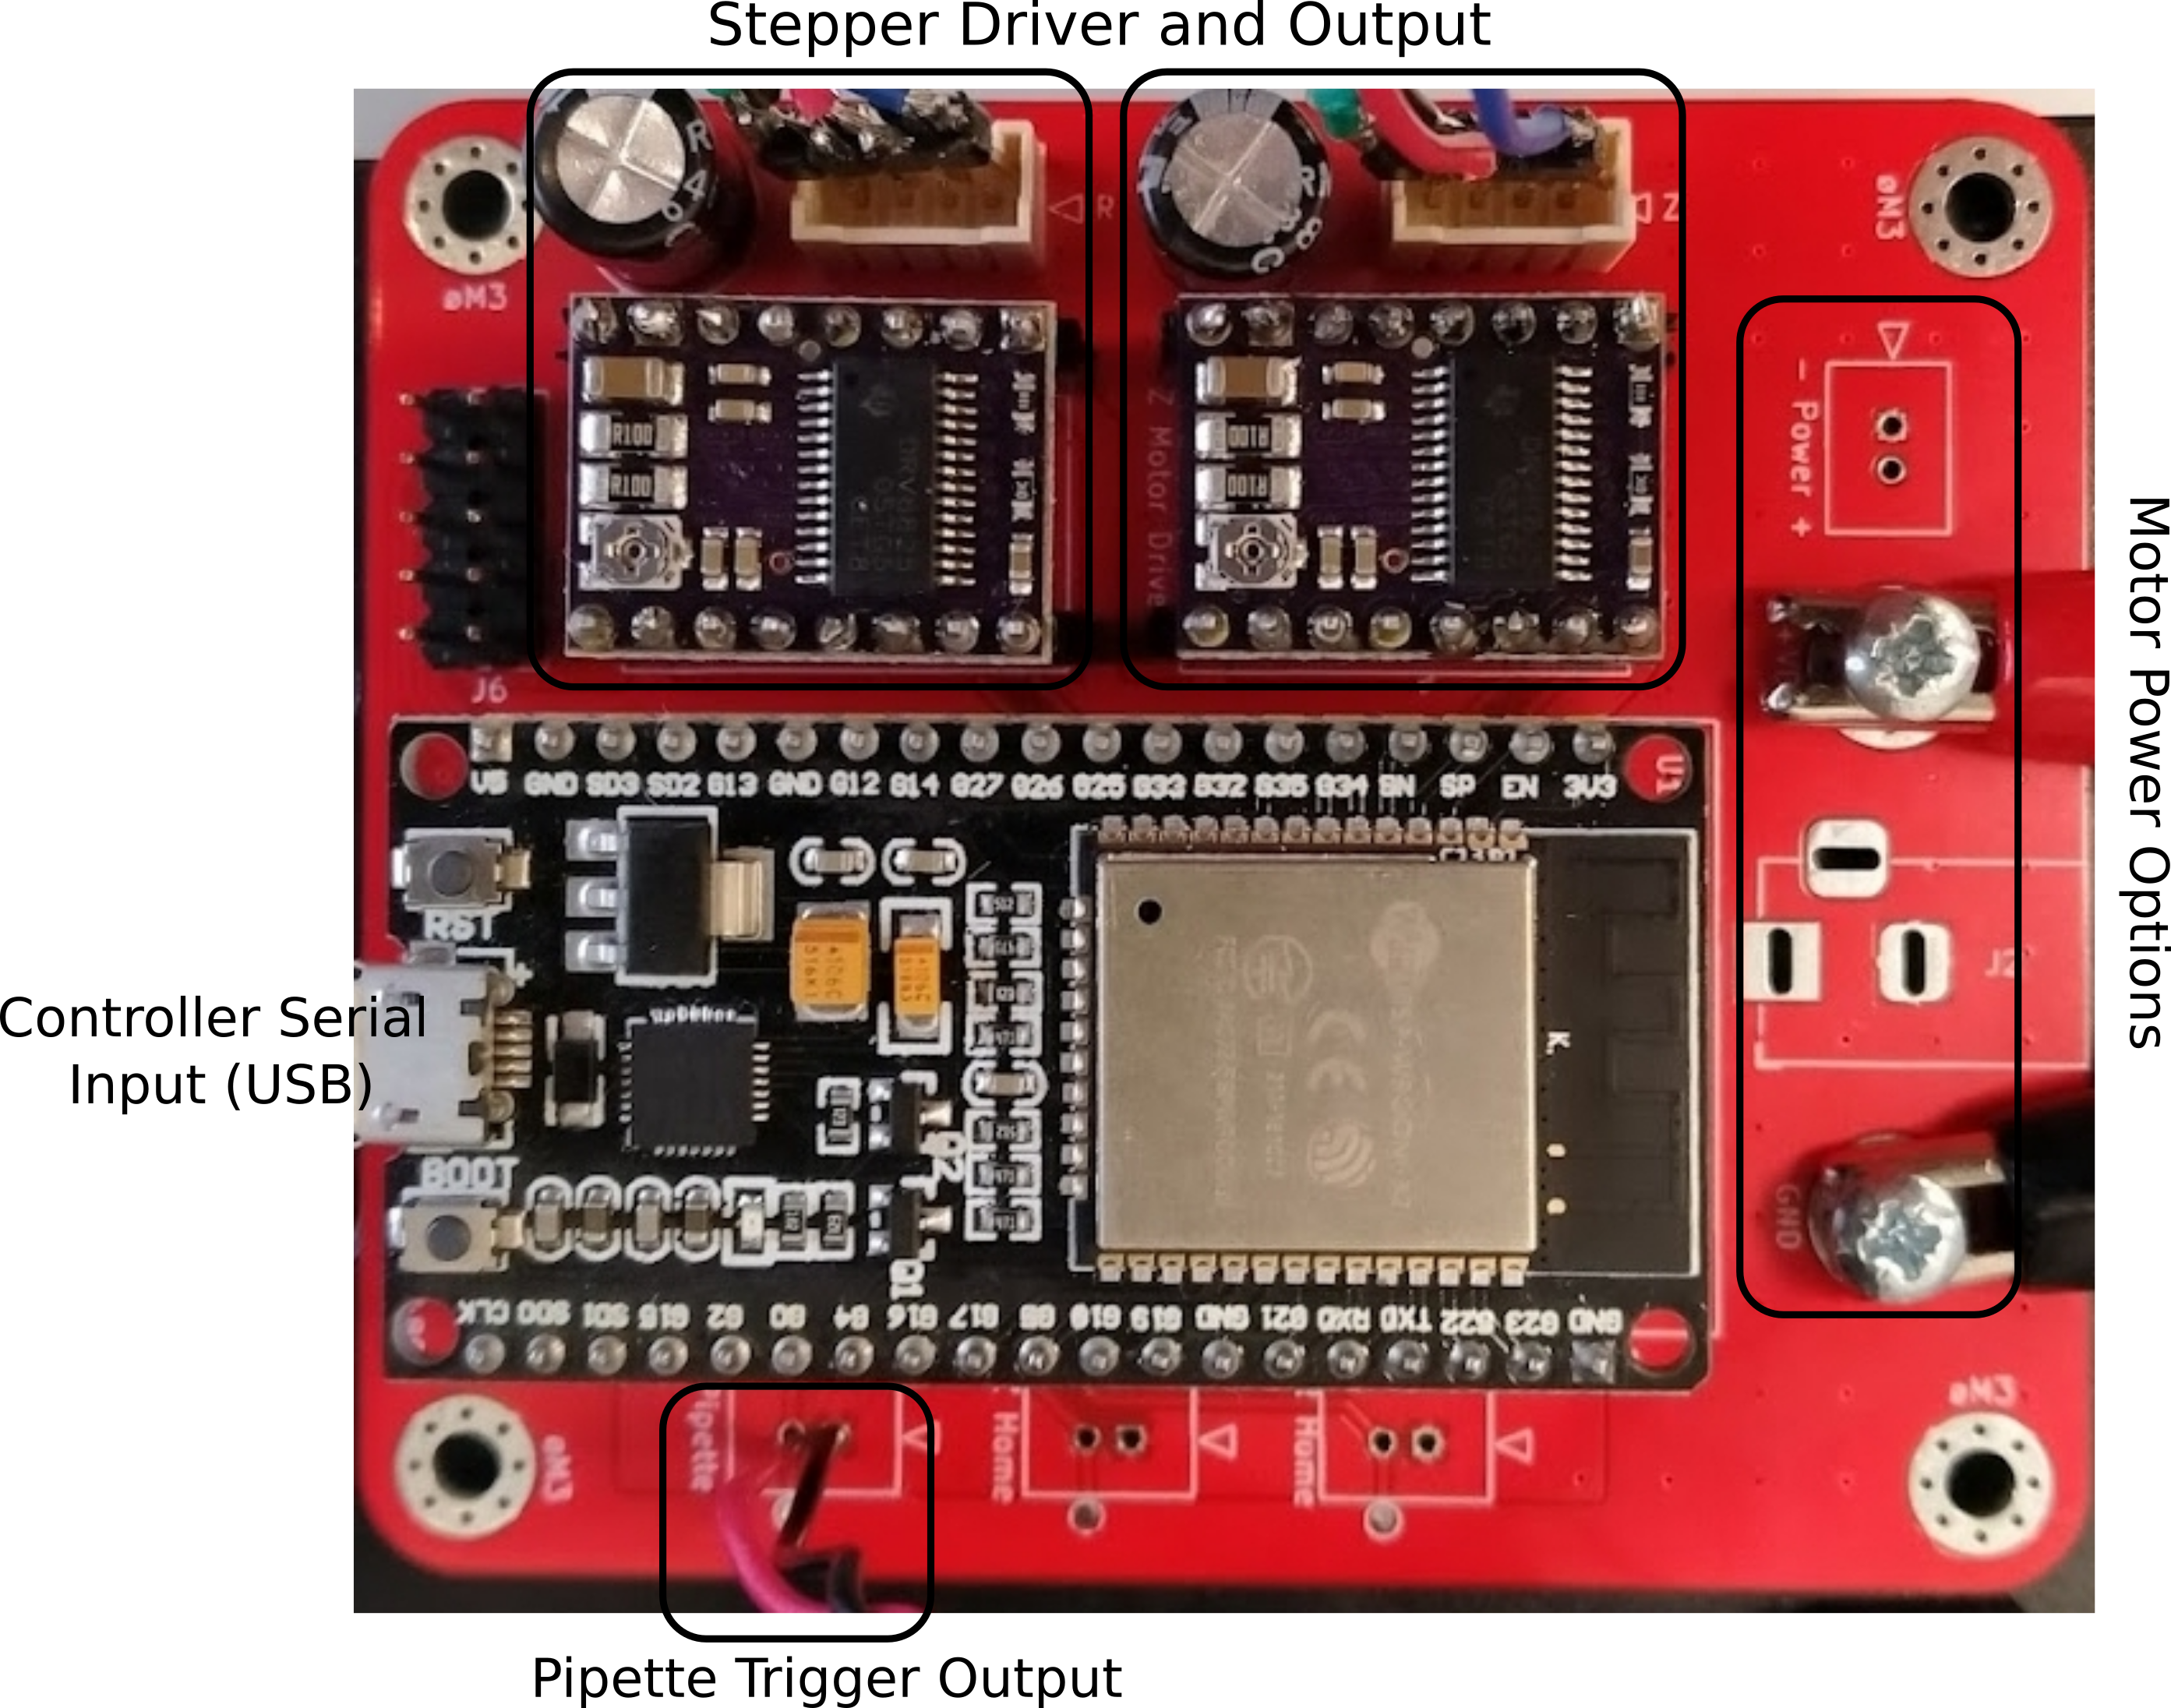
\includegraphics[width=0.4\textwidth]{img/control_pcb.jpg}

\begin{itemize}
    \item full circuit
    \item pcb
    \item any and all adjustment found and made during implementation
\end{itemize}

\subsection{Motor Driving}

\subsection{Setup and Requirements}

\begin{itemize}
    \item characterised skipping issue at 100Hz, 180Hz-200hz in single step
    \item implemted micro stepping to solve
\end{itemize}

//TODO rewrite

Driving firmware was implemented on an ESP32 to validate its ability in producing the required pulse train step signal. The controller was required to produce N steps (pulses) at a set average speed, and ramp up and down that pulse speed at the head and tail of that signal.

Set values of 200 steps forward and back, at a speed of 200 steps per second, with max acceleration or 800 steps per second per second:

These pulses were captured on a second microcontroller listening for falling edges to trigger an interrupt routine to record and display that data.

\subsection{Results}

Figure \ref{fig:code}:a shows a successfully produced signal of 200 pulses with an inferred acceleration at its head/tail. This speed ramping is better illustrated in figure \ref{fig:code}:b showing the stepping change in pulses per second over the course of the pulse train.

\begin{figure}[h]
    \centering
    \begin{subfigure}{.45\textwidth}
        \centering
        \includegraphics[width=0.8\linewidth]{img/stepper_pulses.PNG}
        \caption{Pulse Count}
    \end{subfigure}%
    \begin{subfigure}{.45\textwidth}
        \centering
        \includegraphics[width=0.8\linewidth]{img/stepper_pulse_acc.PNG}
        \caption{Pulses per Second}
    \end{subfigure}
    \caption{}
    \label{fig:code}
\end{figure}

\subsection{Pipette Triggering}
//TODO
\subsection{Environmental Monitoring}
//TODO
\chapter{Evaluation}\label{C:eval}

\section{Mechanical Stability}
Perform Motor driving parameter sweep to optimise mechanical performance according to requirements; 
of minimising pipette tip overshoot and settling time.
\subsection{Procedure}
\begin{itemize}
    \item Position tip at -1/4 revolution before zero point
    \item Set Speed/acceleration values
    \item Swing to zero position
    \item Repeat for value sleep=1rev/s, acc=1/rev/s/s $\rightarrow$  speed=2rev/s, acc=10/rev/s/s
    \item Note: acceleration is the ramp down at end/start of motion so is what we care most about
    \item Camera captured motion 
\end{itemize}

\section{Droplet Volume}
Something the previous system could not achieve was dispensing a variety of volumes.
Use e-pipettes programmable volume to investigate the limits of this project.
\begin{itemize}
    \item How large a droplet can be held on to? (prelim: 8uL)
    \item How large (over above) can reliably self release (w/out touch down)
    \item How small a droplet can be dispensed (e-pipette has draw-back).
\end{itemize}    

\subsection{Results}

//insert generated figures of tip position

//generated trend lines/aggregated data (settle, overshoot) from data.

\section{Repeatability and Reliability}

This section aims to produce the main set of comparable results for evaluating the projects produced system against the output of the previous setup. Thus justifying the success of one of main goals.

\subsection{Procedure}
\begin{itemize}
    \item \textbf{Initial Setup:} Roughly Position substrate stage, reservoir platform and note angular positions as well as vertical clearance requirements.
    \item \textbf{Zero System:} Using overhead camera precisely position pipette tip above substrate centre
    \item \textbf{Data Acquisition:} Initialise cameras, collect pixel:mm calibration data for analysis, initial LabView temperature logger, and environmental monitor noted. Info: temperature data rate, camera frame rate
    \item \textbf{Automated Sequence:} Via the serial link, enter the procedures command sequence to represent $\rightarrow$ lower, draw up fluid, raise, position over substrate, dispense, lower, raise, clear camera view. With appropriate delays.
    \item \textbf{Capture:} Begin data collection and automated dispense.
    \item \textbf{Repeat: } Minimum of 5 times. Each time carefully cleaning substrate surface to minimised up measured factors. 
\end{itemize}

\subsection{Analysis}

To show the system successfully increases the consistency of droplet position,
\chapter{Conclusions and Future Work}\label{C:conclusion}

\section{Conclusions}

The aims of this project were to control for variations in droplet morphology; droplet position and volume, providing an improvement over the previous system. Produce an extendable platform that enabled the experimental process to be automated/centrally controlled to speed up the procedure. Provide a data collection system for uncontrolled factors. 
These goals were chosen with the hypothesis that improving the system's performance in these aspects would carry through to an improvement in the inconsistent results observed in the previous iteration of the system.  

To control for droplet volume and provide a method for variable volume, this project utilised a pre-calibrated electronic pipette as the central droplet dispensing tool that is interfaced with to provide remote GPIO control. Automation, user control and positional control was achieved via a serial command-driven stepper motor controller that drove the motion of a micrometer controlled XYZ stage mounted upon an optical breadboard.   

\subsection*{Successes}
The use of a pre-calibrated electronic pipette eliminates volume variation to a point beyond the scope of this projects ability to measure, but more importantly, the mechanical system was confirmed to be stable enough to support the full variable volume range from 0.5 to 10 microlitres.

The stepper motor driving system parameters were successfully tuned to reduced pipette tip settling oscillation below 1mm in 1s and achieves consistent and exact positioning. This precision in instrumentation control resulted in the reduction in droplet positional offset  variance from 0.296mm to 0.018mm.

From initial analysis of the collected temperature profiles, this project can preliminarily confirm the hypothesis that improved positional and volume consistency will result in greater consistency in experimental results. Though more data is needed.

The firmware and controller implemented fully supports input of predefined command sequences that allows a user to quickly run the same complex experimental procedure much time, with the exact same instrumentation performance.   

\subsection*{Drawbacks}
Major drawbacks of the resulting design include the XY positional locking of the pipette stage due to static Z motor mounting on the breadboard. This results in any required adjustment to the camera, substrate and reservoir to be carried out to fit the pipette stage position.

This implementation lacks auto-homing to set zero position, and additionally due to the permanent magnetic pole of the stepper motor stator combined with the drivers micro steppers, the user can request an invalid holding position as home. This cannot be maintained due to current limits and will snap away from it. This should however be evident in the setup stage of the experiment.  

\section{Future Work}
As stated this project produced an extendable platform from which a variety of features can be implemented.
\begin{itemize}
    \item User-Friendly Graphical Control to interface with serial command controller. As of now, there exists a LabVIEW script that can interface with the serial input of the controller but more in-depth user-friendly version would be a great step up in the usability of the system.
    \item Due to the projects nature combined with an inopportune COVID19 lockdown the integration of homing switches to automate setup was planned but not implemented. This addition would increase setup speed and usability.
    \item Utilise included GPIO breakout header to synchronise external data acquisition
    \item Further investigate Temperature evolution with varied volume, substrates, cleaning techniques
    \item Add enclosure to isolate air currents and further control variables.
\end{itemize}

%%%%%%%%%%%%%%%%%%%%%%%%%%%%%%%%%%%%%%%%%%%%%%%%%%%%%%%

\backmatter

%%%%%%%%%%%%%%%%%%%%%%%%%%%%%%%%%%%%%%%%%%%%%%%%%%%%%%%

\bibliographystyle{ieeetr}
\bibliography{bib}

\end{document}
